

\documentclass[12]{fphw}
\usepackage{float}
% Template-specific packages

\usepackage{graphicx} % Required for including images



\usepackage{fullpage,enumitem,amsmath,amssymb,graphicx}
\usepackage{pdfpages}
\usepackage{amsmath} 
% for table
\newcommand\Tstrut{\rule{0pt}{2.6ex}}       % "top" strut
\newcommand\Bstrut{\rule[-0.9ex]{0pt}{0pt}} % "bottom" strut
\newcommand{\TBstrut}{\Tstrut\Bstrut} % top&bottom struts
\usepackage{fancyhdr}
\pagestyle{fancy} 
\setlength{\headheight}{10pt}


%----------------------------------------------------------------------------------------
%	ASSIGNMENT INFORMATION
%----------------------------------------------------------------------------------------

\title{Homework \#1} % Assignment title

\author{Ali BaniAsad} % Student name

\date{April 9th, 2021} % Due date

\institute{Sharif University of Technology \\ Institute of Aerospace} % Institute or school name

\class{Flight Dynamic II} % Course or class name

\professor{Dr.Zare} % Professor or teacher in charge of the assignment

%----------------------------------------------------------------------------------------

\begin{document}
	
	\maketitle % Output the assignment title, created automatically using the information in the custom commands abov
	\section*{Problem 1}
	\begin{enumerate}[label=(\alph*)]
		\item 
		The Earth-center, Earth-fixed(ECEF) frame:


In specific time origins of ECEF fix to earth centered inertial(ECI) frame and we assume in 100 second they don't change too much so we neglect this change.


$u^i(t) = u^i_o + a^i_xt,\quad v^i(t) = a^i_yt, \quad w^i(t) = 0$



$u_o^i = 100 ft/s,\quad a_x^i = 25 ft/s^2, \quad a_y^i = 50ft/s^2$

$$u^i(t) = 100 + 25t,\quad v^i(t) = 50t, \quad w^i(t) = 0$$
$$x^i(t) = 100t + 25/2t^2,\quad v^i(t) = 50/2t^2, \quad w^i(t) = 0$$

Figures have plot in MATLAB and code(Q1\_a) attached to home work file.
\begin{figure}[H]
	\caption{X location ECEF frame}
	\centering
	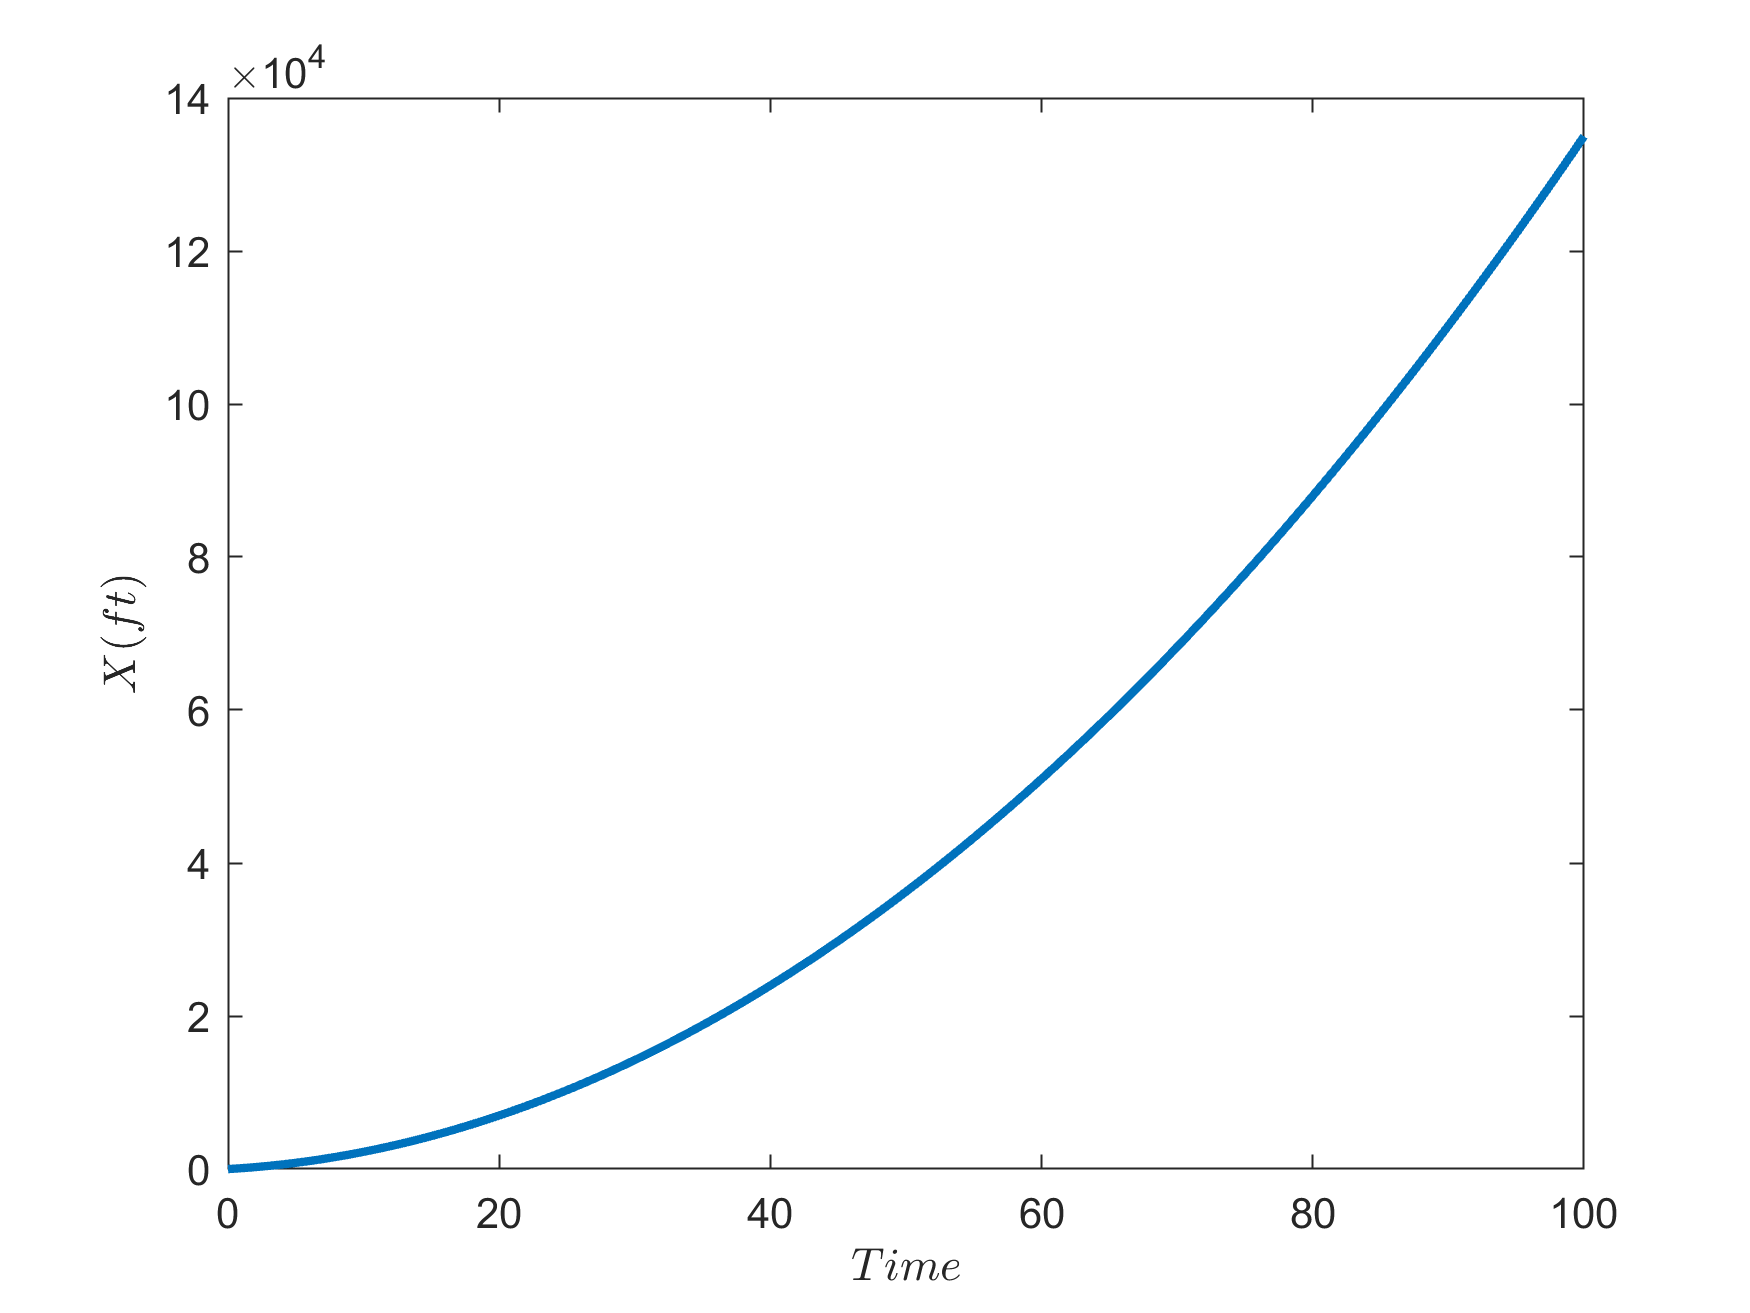
\includegraphics[width=12cm]{Q1/figures/X location.png}
\end{figure}
\begin{figure}[H]
	\caption{Y location ECEF frame}
	\centering
	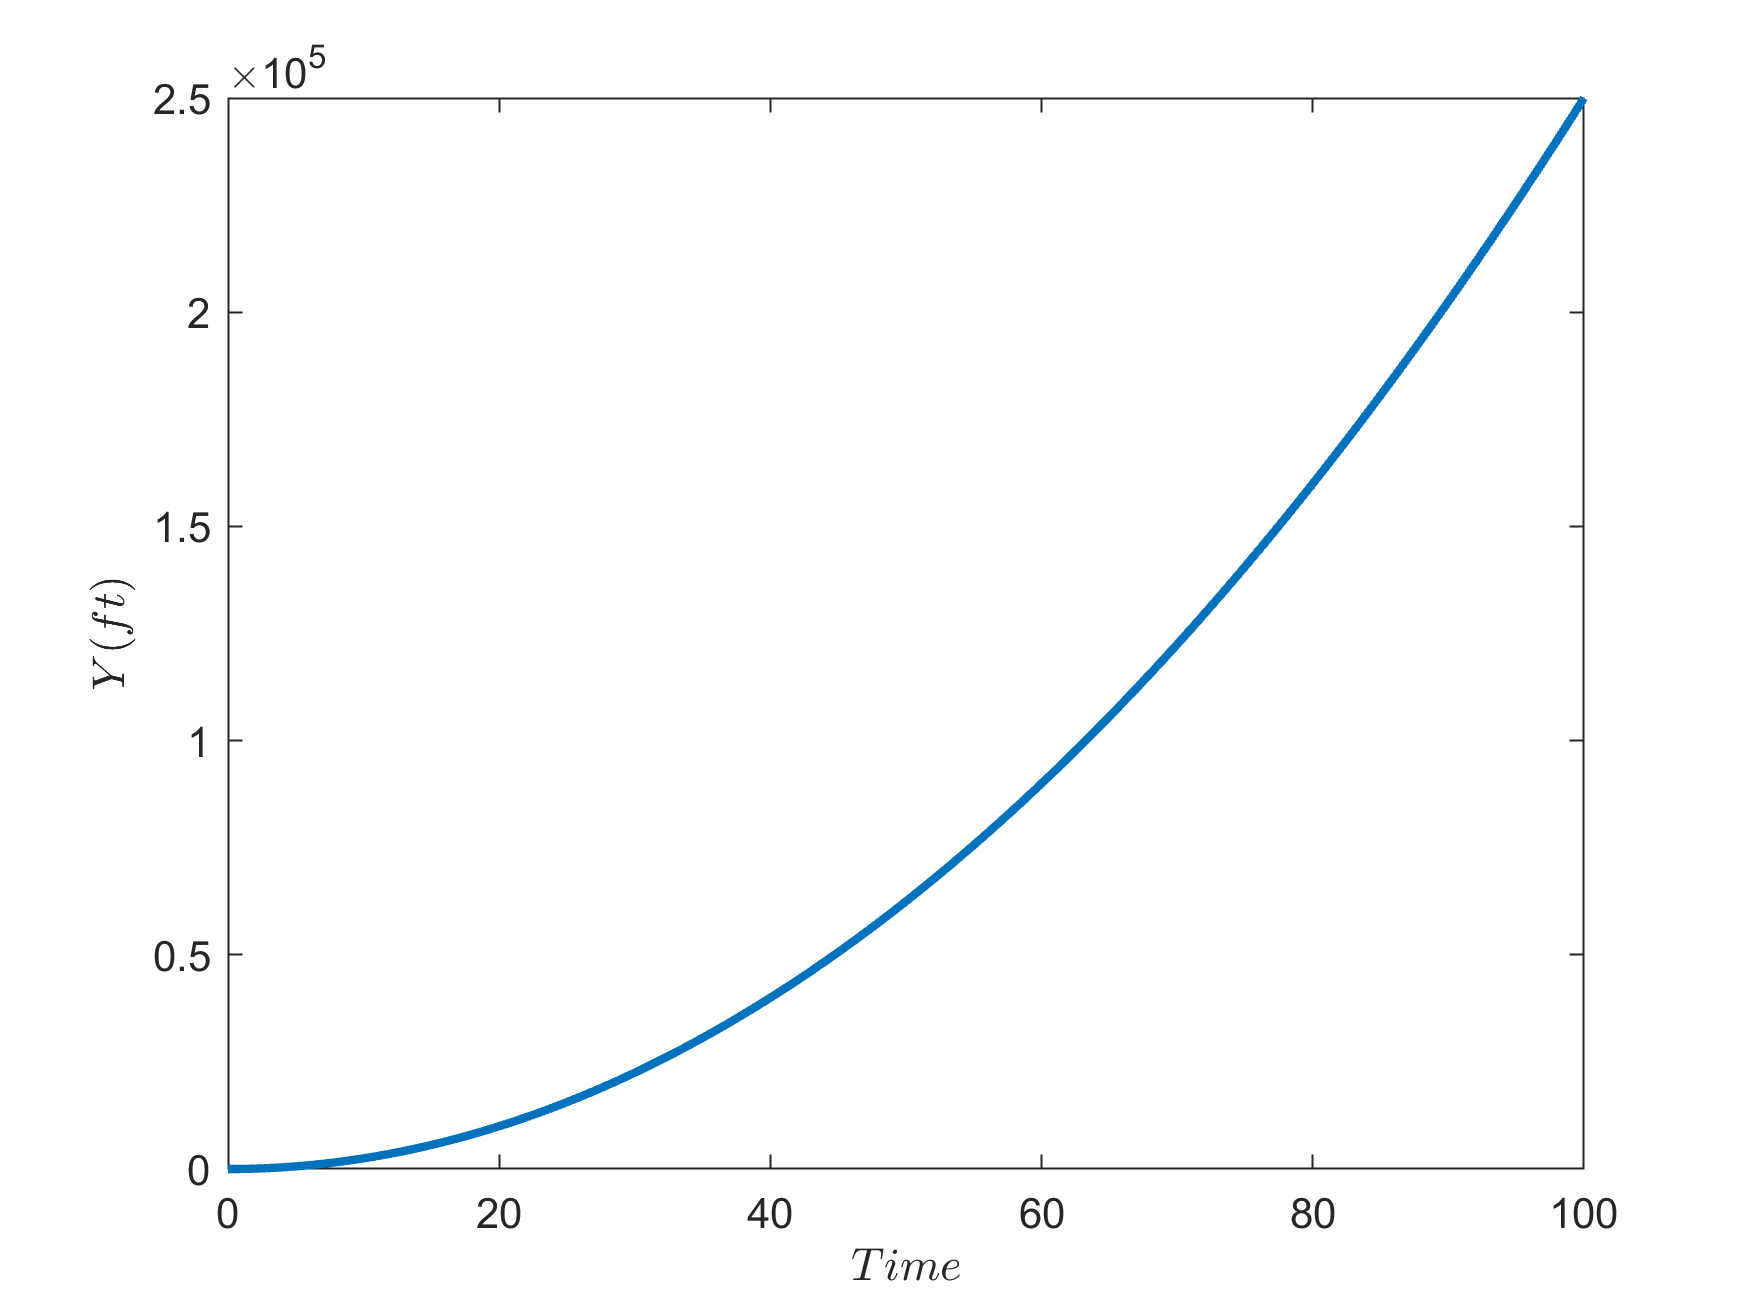
\includegraphics[width=12cm]{Q1/figures/Y location.png}
\end{figure}
\begin{figure}[H]
	\caption{Z location ECEF frame}
	\centering
	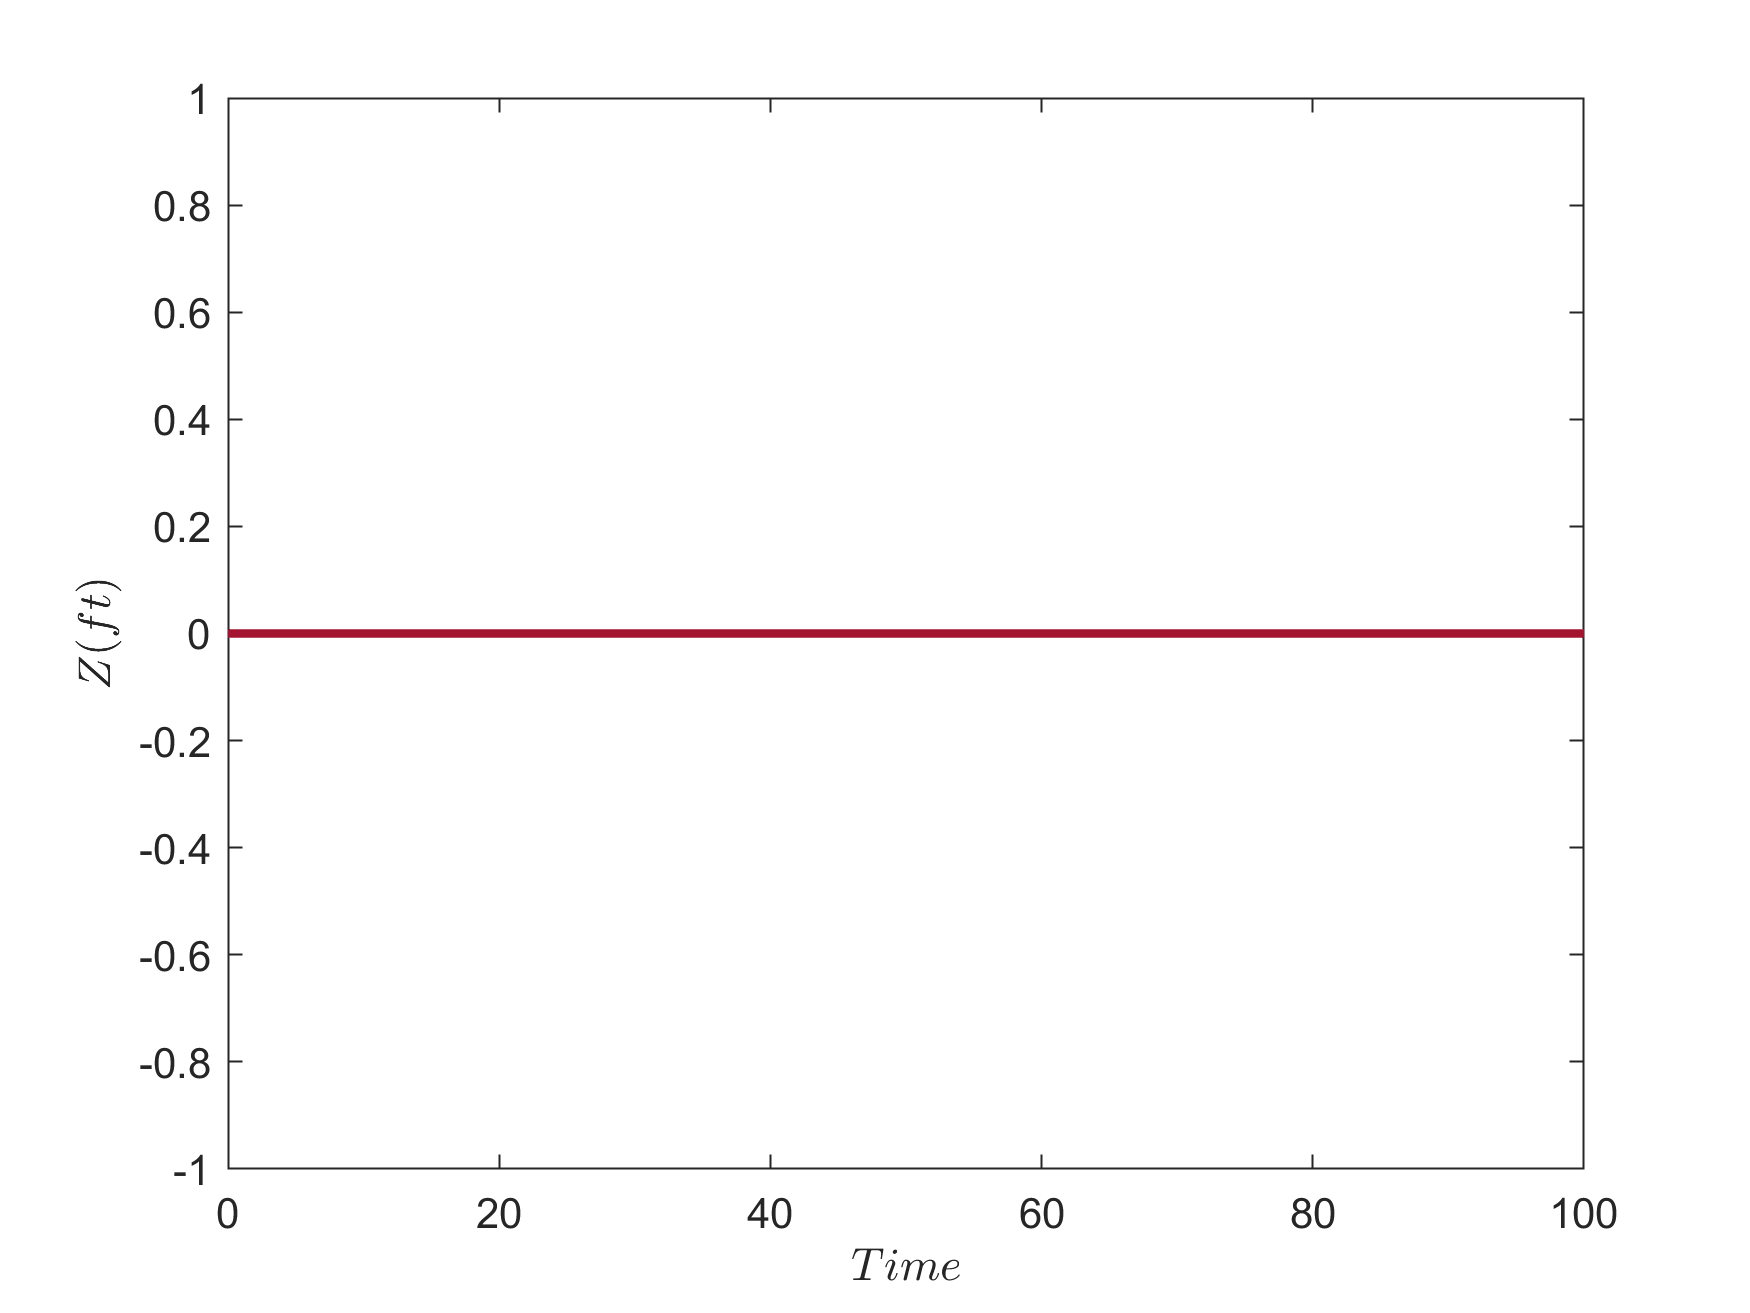
\includegraphics[width=12cm]{Q1/figures/Z location.png}
\end{figure}
\begin{figure}[H]
	\caption{X direction velocity ECEF frame}
	\centering
	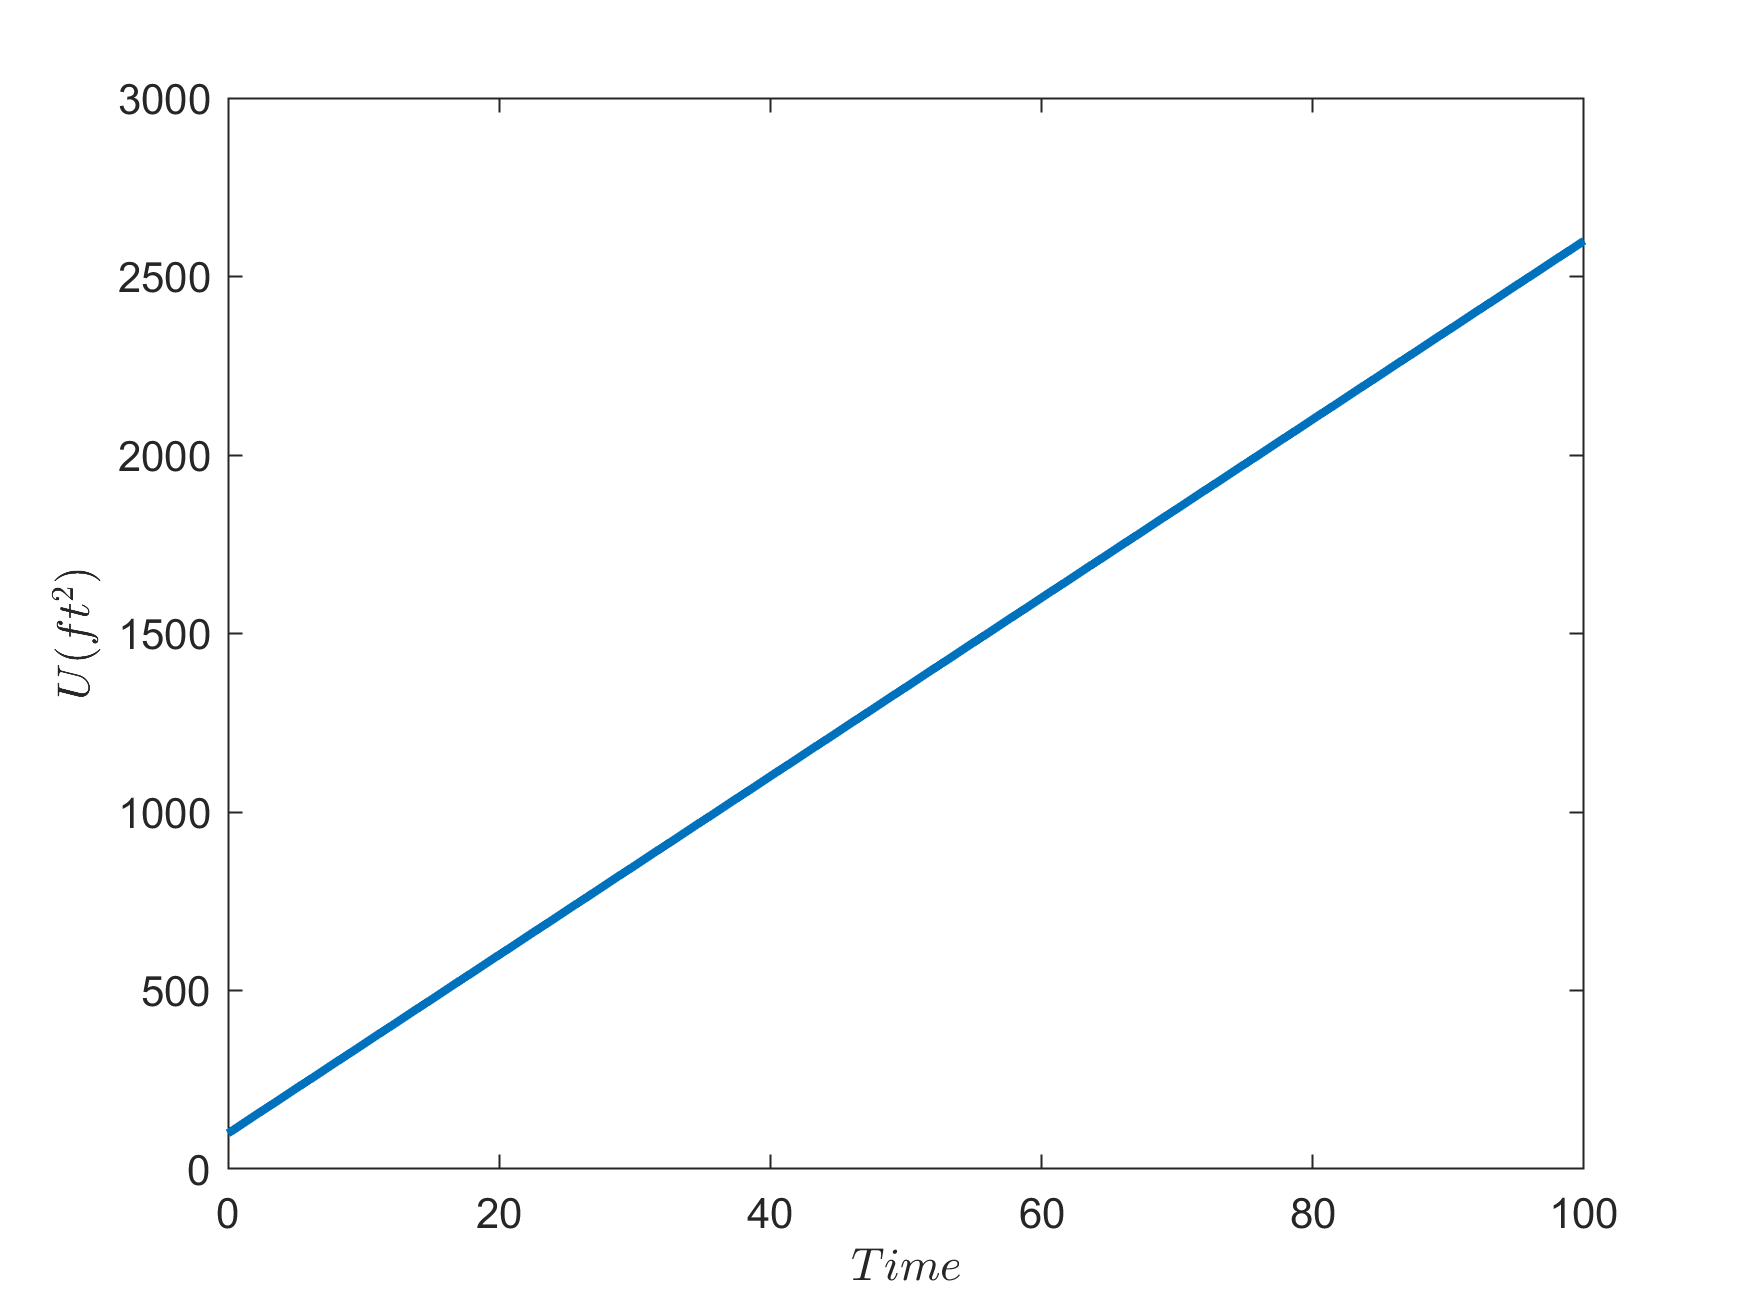
\includegraphics[width=12cm]{Q1/figures/X velocity.png}
\end{figure}
\begin{figure}[H]
	\caption{Y direction velocity ECEF frame}
	\centering
	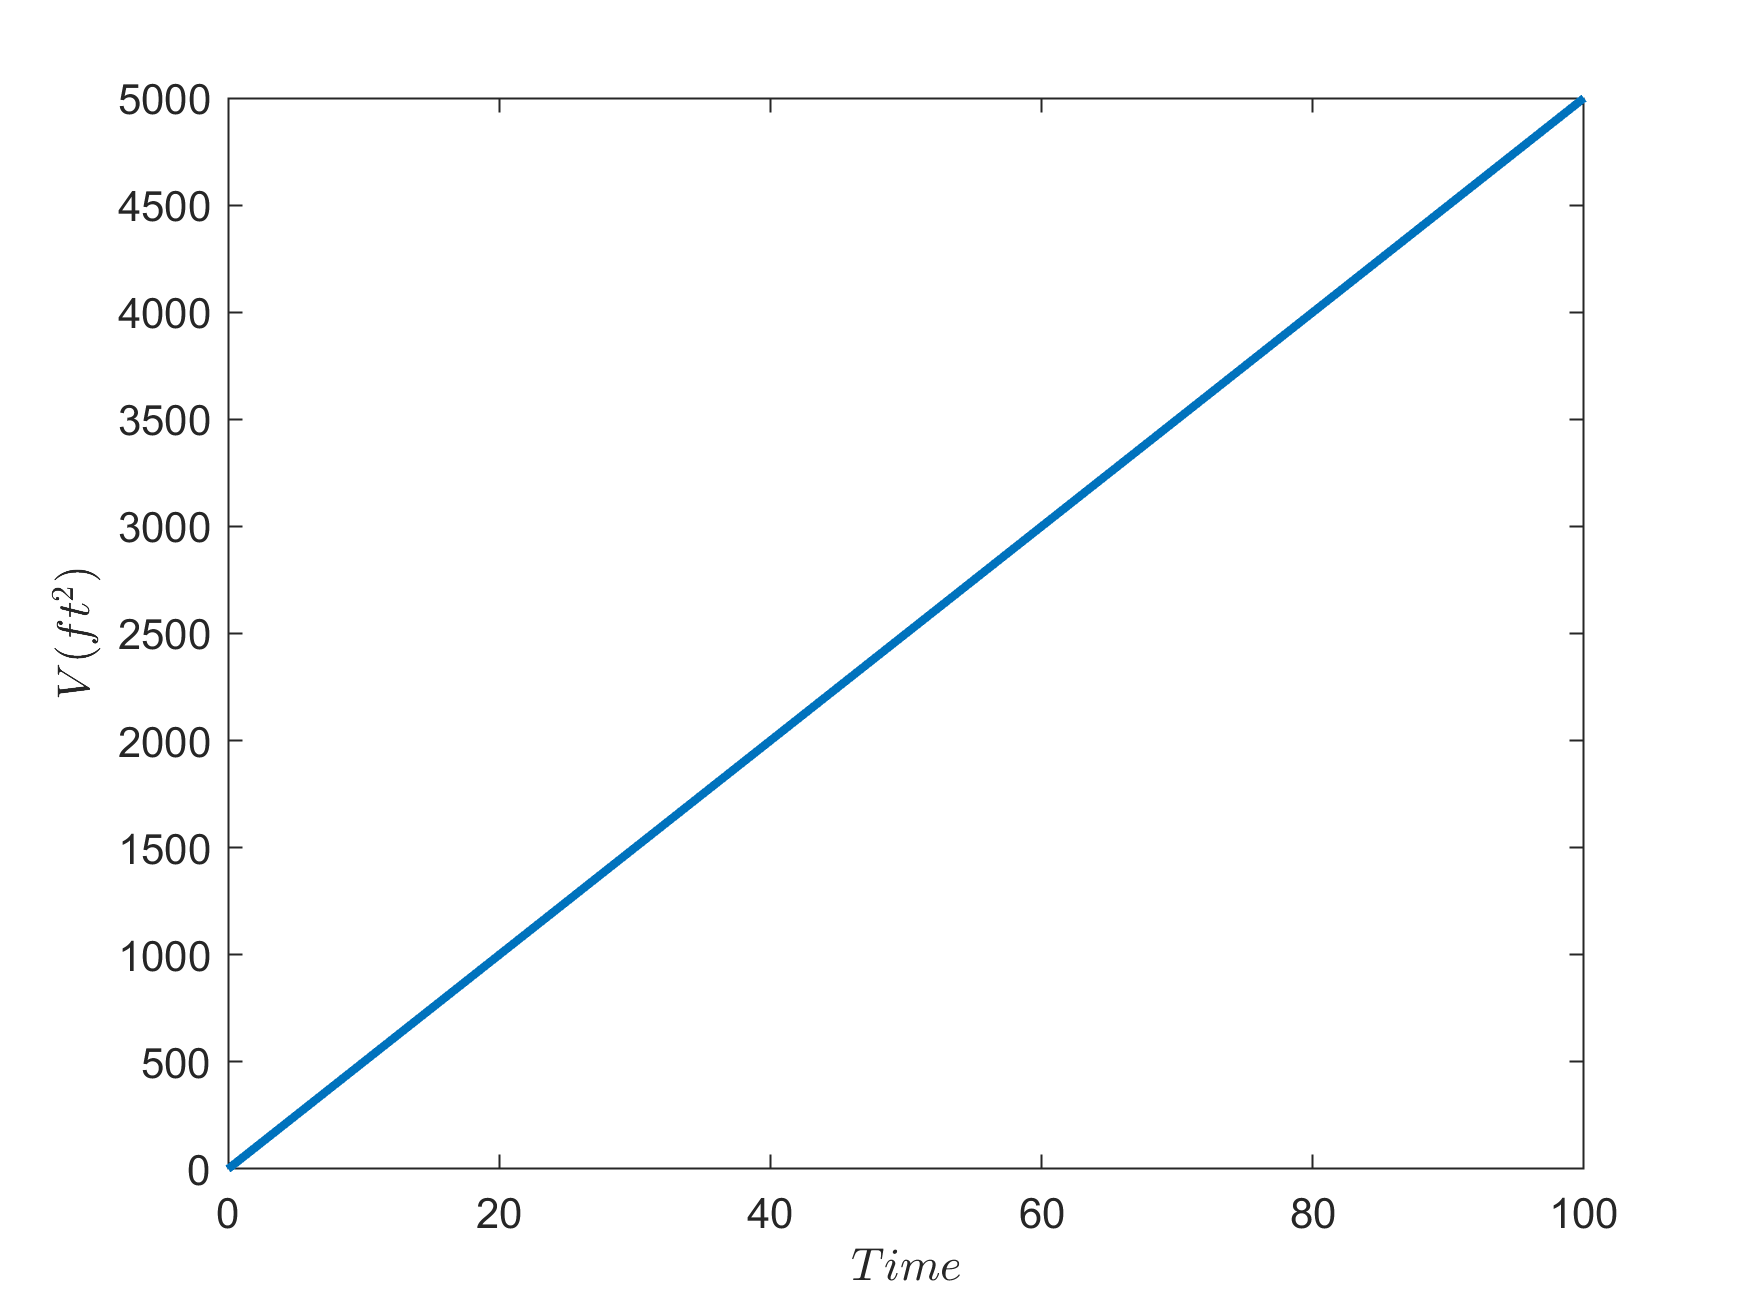
\includegraphics[width=12cm]{Q1/figures/Y velocity.png}
\end{figure}
\begin{figure}[H]
	\caption{Z direction velocity ECEF frame}
	\centering
	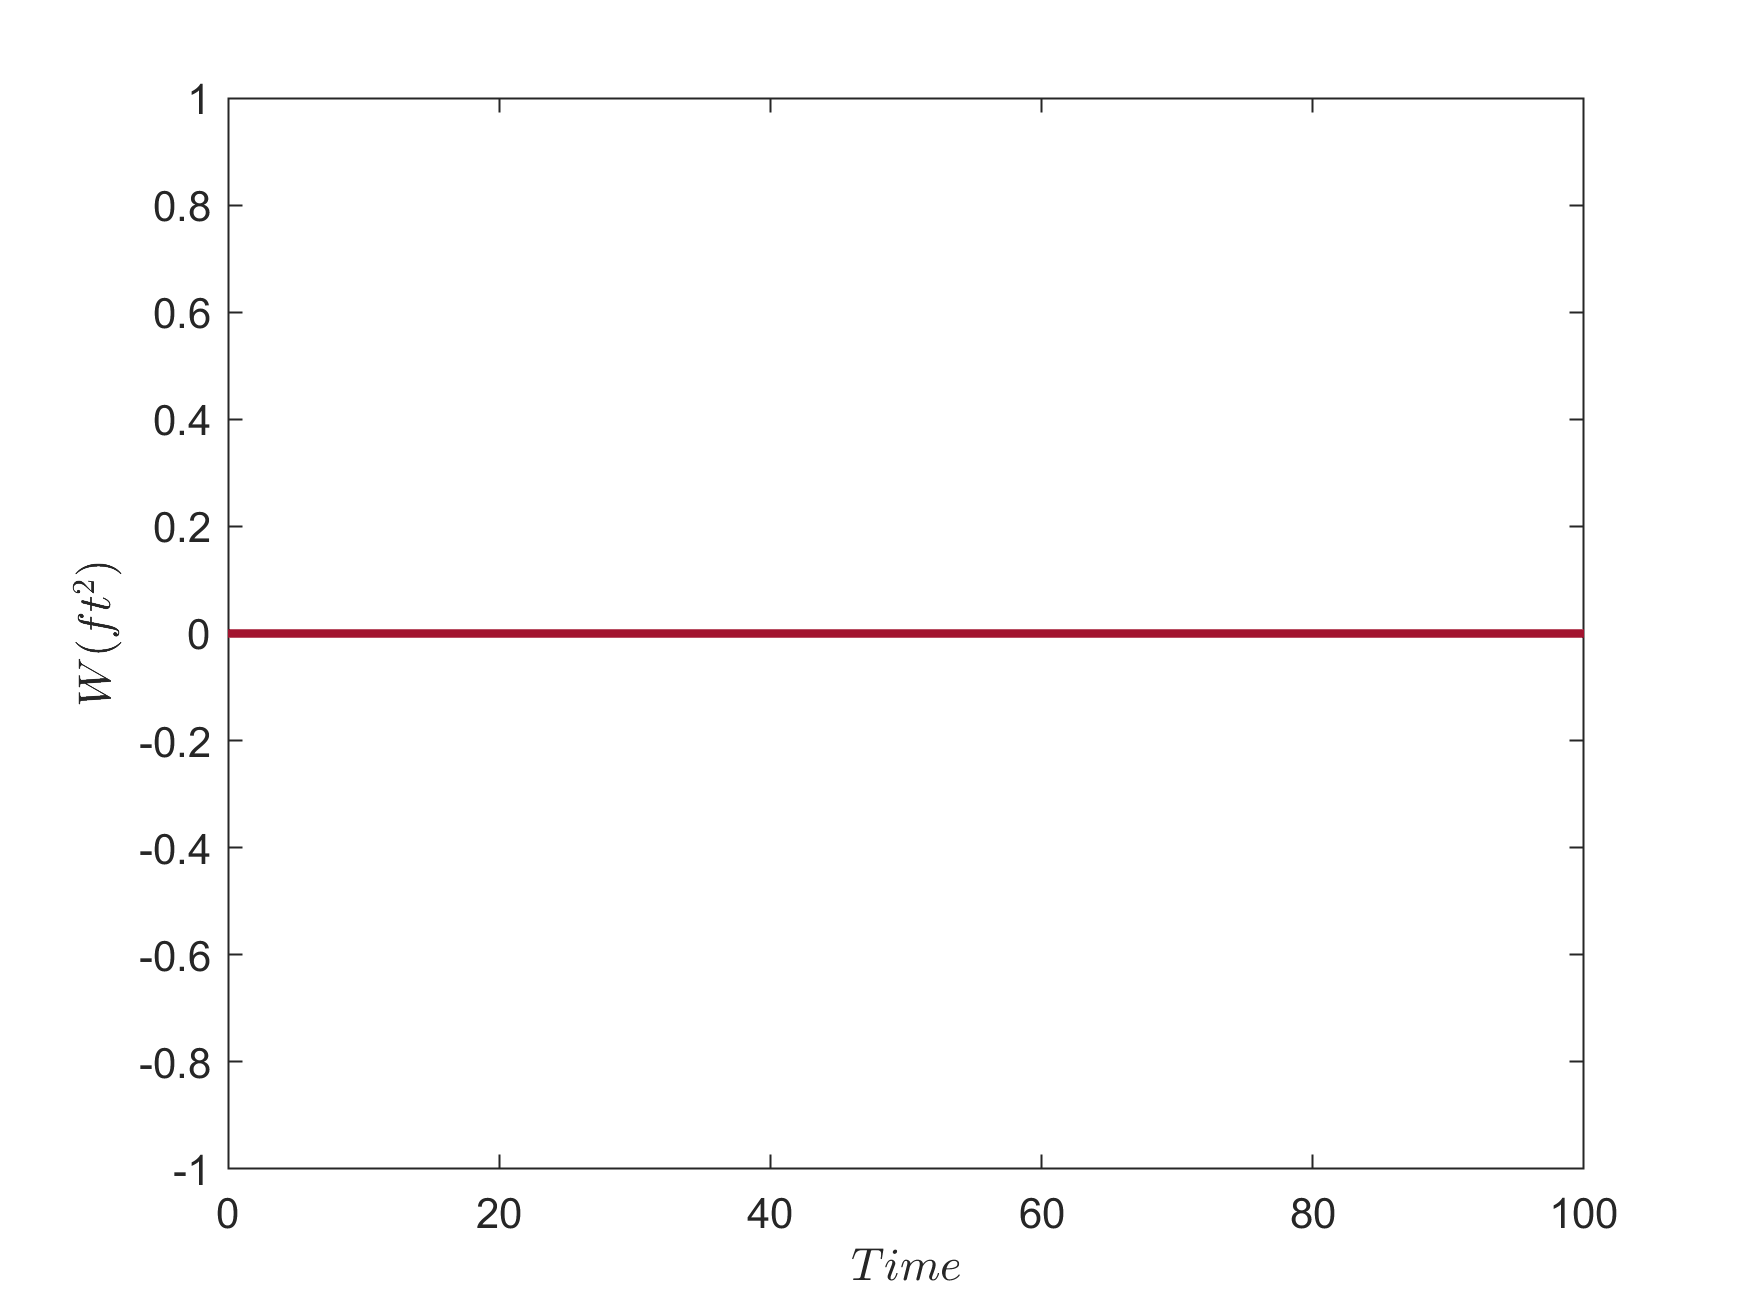
\includegraphics[width=12cm]{Q1/figures/Z velocity.png}
\end{figure}
		\item 
		kos
	\end{enumerate}
	\section*{Problem 2}
	\begin{enumerate}[label=(\alph*)]
		\item 
		Body to tunnel transformation matrix:
\\
Angle of attack:
$$\theta = 20^{\circ}$$
Yaw angle:
$$\psi = 10^{\circ}$$
Bank angle:
$$\phi = 10^{\circ}$$

$$R_{body}^{tunnel} = \begin{bmatrix}
	\cos(-\psi) & -\sin(-\psi) & 0 \\
	\sin(-\psi) & \cos(-\psi)  & 0 \\
	0          &     0       & 1
\end{bmatrix} \times
\begin{bmatrix}
	\cos(-\theta) & 0 & \sin(-\theta)   \\
		0      & 1  &       0 \\
	-\sin(-\theta) & 0 & \cos(-\theta)  

\end{bmatrix} \times
\begin{bmatrix}
		1      & 0 &         0     \\
	0 & \cos(-\phi) &  -\sin(-\phi)   \\

	0 &  \sin(-\phi) & \cos(-\phi)  
	
\end{bmatrix}  $$

$$R_{body}^{tunnel} = \begin{bmatrix}
	    0.9254  &  0.2295  & -0.3016 \\
		-0.1632  &  0.9595  &  0.2295 \\
		0.3420  & -0.1632  &  0.9254 \end{bmatrix}$$
		\item 
		Transfer from body to stability:
\newline
$$\begin{bmatrix}
	-D \\
	 Y \\
	-L
\end{bmatrix}^S = R_B^S \times
\begin{bmatrix}
	F_X \\
	F_Y \\
	F_Z
	\end{bmatrix}^B $$
$$R_B^S = 
\begin{bmatrix}
	\cos(\theta) & 0 & \sin(\theta)   \\
	0      & 1  &       0 \\
	-\sin(\theta) & 0 & \cos\theta)  
\end{bmatrix}
\times
\begin{bmatrix}
	1      & 0 &         0     \\
	0 & \cos(\phi) &  -\sin(\phi)   \\
	
	0 &  \sin(\phi) & \cos(\phi)  
	
\end{bmatrix} 
$$
Transformation matrix:
$$R_B^S = \begin{bmatrix}
	    0.9397   & 0.0594  &  0.3368 \\
	0  &  0.9848  & -0.1736 \\
	-0.3420  &  0.1632  &  0.9254
\end{bmatrix}$$
$$F^S = \begin{bmatrix}
	  -12.2196\\
	-16.6967\\
	-97.0196\\
\end{bmatrix}$$

	\end{enumerate}
	\section*{Problem 3}
	\begin{enumerate}[label=(\alph*)]
		\item
		Oooooooooooooops
		\item 
		File of Simulink Attached to home work.
	\end{enumerate}


	

\end{document}
